\clearpage
\subsection{Caso 6. UDP: reflexión/amplificación DNS, NTP o SSDP}
\label{caso:udp-reflexion}

\begin{situacion}
El servidor o gateway registra un volumen inusual de respuestas UDP, posiblemente desproporcionado respecto de las solicitudes. En la reflexión, el atacante falsifica la dirección de origen y envía la petición a un servicio que responde a la víctima; en la amplificación, la respuesta es mayor que la petición, de modo que el atacante multiplica el tráfico con poco esfuerzo.

\textbf{Objetivo:} \par
Reproducir en el laboratorio la reflexión y la amplificación con DNS, NTP y SSDP, medir el factor de amplificación de cada protocolo, compararlo con una línea base legítima y proponer controles del lado del servidor y de la red.

\textbf{Fundamento teórico:} \par
Los tres protocolos comparten un patrón: viajan sobre UDP, no verifican el origen y responden a cualquiera. DNS puede devolver respuestas muy grandes (TXT, ANY o DNSSEC) a consultas pequeñas; la amplificación por DNS es una de las más estudiadas y sigue vigente incluso con servidores que ya no son recursivos abiertos \parencite{nawrocki2021farside,koch2025forward}. NTP incluye un comando privado de monitoreo, \textit{monlist} (modo~7), que devolvía hasta 440~bytes por una petición de 52~bytes; ntpd lo deshabilitó por defecto en la versión 4.2.7p26 y el protocolo se documenta en el RFC~5905 \parencite{rfc5905}. SSDP, el descubrimiento de dispositivos UPnP, responde a un \texttt{M-SEARCH} con una respuesta por dispositivo, de modo que una sola petición puede generar varias respuestas. La defensa tiene dos frentes: cerrar o limitar el servicio que amplifica y filtrar el tráfico con origen falsificado en la red de origen \parencite{nawrocki2023sok,kopp2021ddos}.

El punto crítico es que la IP de origen falsificada hace que la víctima reciba tráfico que nunca solicitó y que el atacante quede oculto. Sin filtrado de origen (BCP~38) en la red del atacante, el fenómeno no se puede eliminar desde la víctima.
\end{situacion}

\paragraph{Procedimiento.}
Se reutilizó la red aislada \texttt{172.28.50.0/24}. Se agregó un reflector didáctico en \texttt{172.28.50.53} que responde DNS/53, NTP/123 y SSDP/1900, y se mantuvo un host pasivo en \texttt{172.28.50.20} como víctima. El analista en \texttt{172.28.50.10} generó el tráfico con Scapy y falsificó el origen para que las respuestas llegaran a la víctima. Nada salió de la red del laboratorio. El procedimiento fue:

\begin{enumerate}
	\item \textbf{Integridad:} se calcularon las huellas SHA-256 de las cinco capturas antes de analizarlas (Figura~\ref{fig:c6_hashes}).
	\item \textbf{Línea base:} diez consultas DNS a \texttt{www.lab.local}, una consulta NTP de cliente (48~bytes) y un \texttt{M-SEARCH} SSDP legítimo, todos desde el analista y con origen real.
	\item \textbf{Amplificación DNS:} 120 consultas TXT a \texttt{big.lab.local} con origen falsificado \texttt{172.28.50.20}; el reflector devuelve un TXT de 2.455~bytes que, con las cabeceras, ocupa dos fragmentos IP (Figura~\ref{fig:c6_dns}).
	\item \textbf{NTP monlist:} 40 consultas privadas de modo~7 con código~42 y origen falsificado; el reflector emula la respuesta de 440~bytes (Figura~\ref{fig:c6_ntp}).
	\item \textbf{SSDP:} 40 \texttt{M-SEARCH} con origen falsificado; el reflector emula cuatro dispositivos y responde cuatro veces por petición (Figura~\ref{fig:c6_ssdp}).
	\item \textbf{Dos puntos de captura:} el reflector conservó una captura continua que se recortó por fase con \texttt{tshark}, y la víctima conservó su propia captura pasiva. La segunda fuente es independiente de la primera y permite comprobar que el tráfico llegó sin haber sido solicitado.
	\item \textbf{Análisis y IDS:} el script \texttt{analyze\_cu6.py} calculó peticiones, respuestas, bytes por dirección, factor de amplificación, fragmentación y víctimas únicas; las capturas se reprocesaron con Suricata~7.0.7.
\end{enumerate}

\begin{figure}[H]
	\centering
	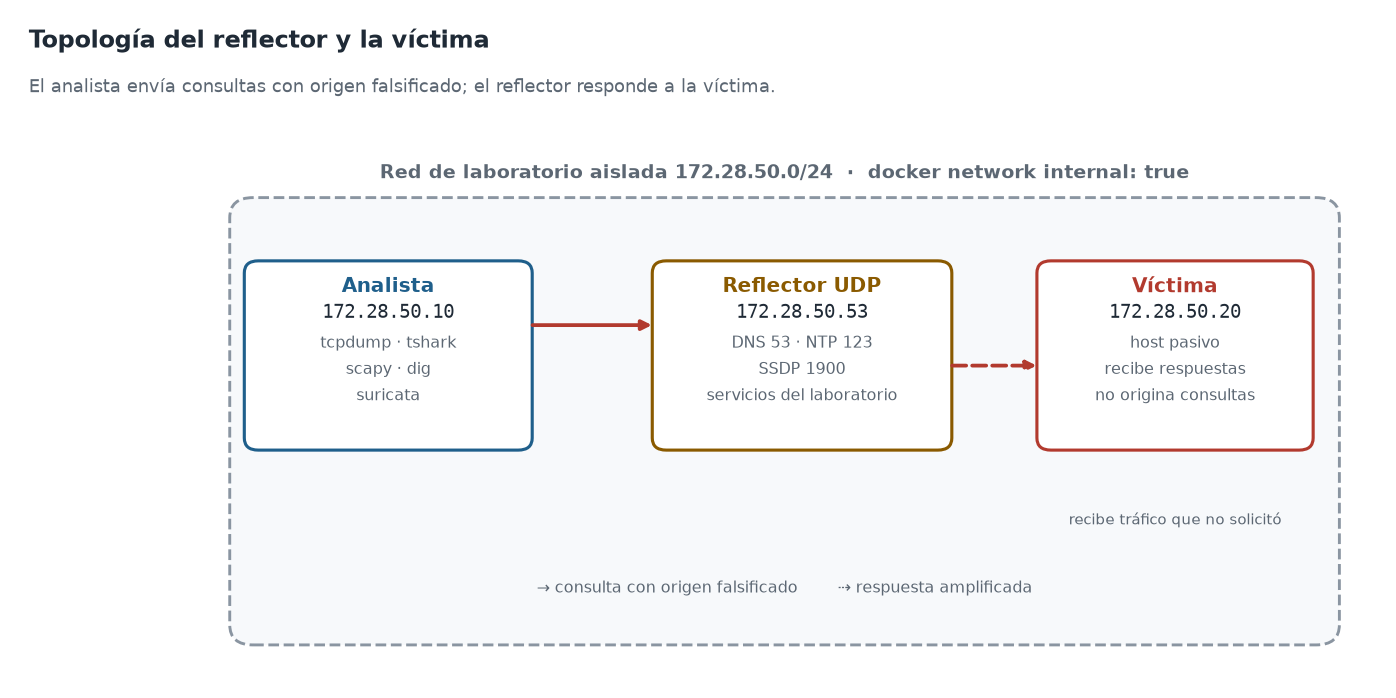
\includegraphics[width=0.95\textwidth]{imagenes/Evidencias CU-6/01_topologia_lab.png}
	\caption{Topología del reflector y la víctima en el Caso 6.}
	\label{fig:c6_topologia}
\end{figure}

\begin{figure}[H]
	\centering
	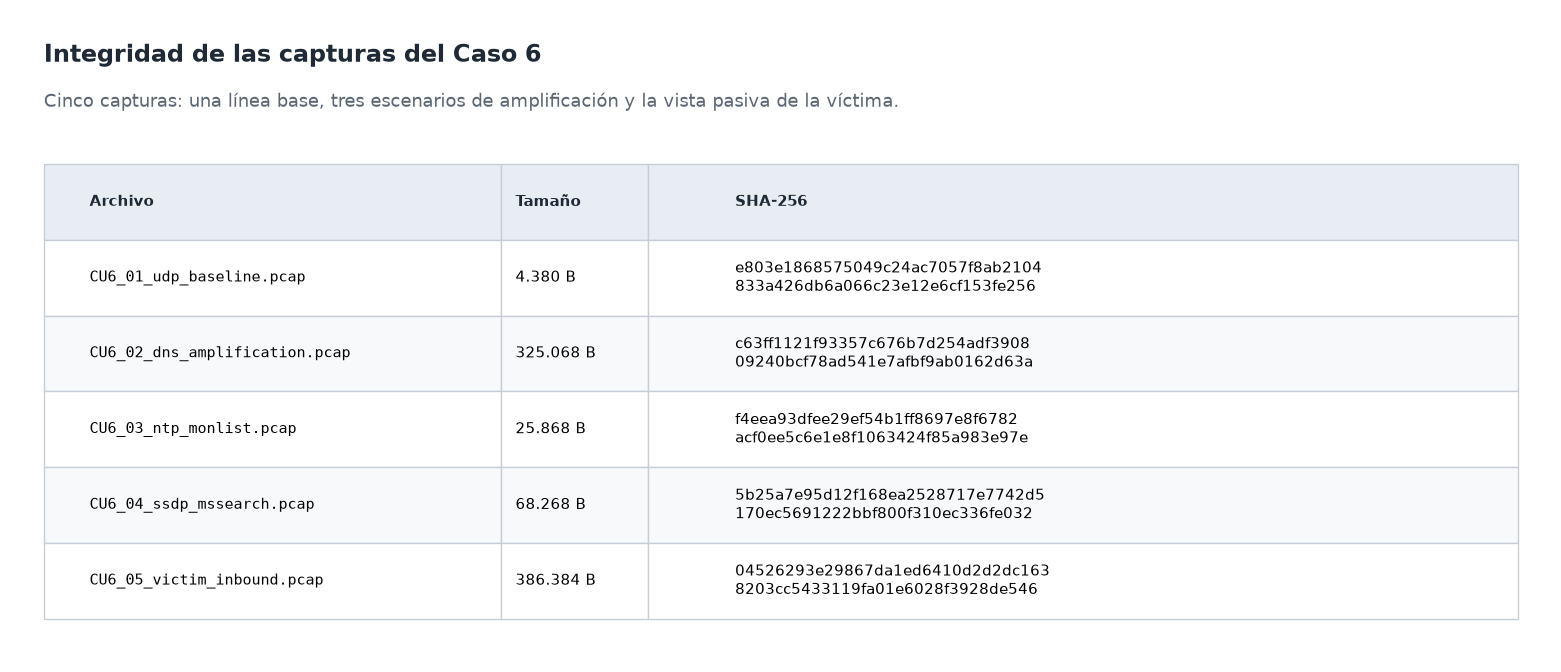
\includegraphics[width=0.92\textwidth]{imagenes/Evidencias CU-6/02_hashes_sha256.png}
	\caption{Verificación de integridad de las capturas del Caso 6 mediante SHA-256.}
	\label{fig:c6_hashes}
\end{figure}

\begin{figure}[H]
	\centering
	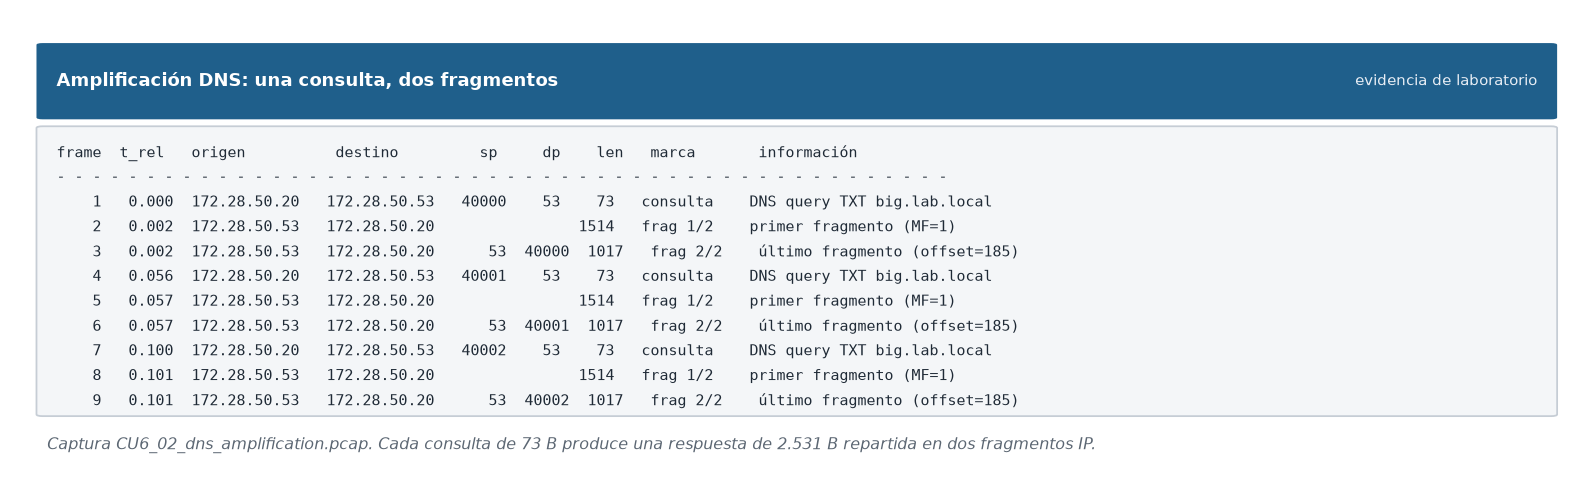
\includegraphics[width=0.98\textwidth]{imagenes/Evidencias CU-6/03_dns_amplificacion.png}
	\caption{Amplificación DNS: una consulta de 73~bytes y una respuesta de 2.531~bytes en dos fragmentos.}
	\label{fig:c6_dns}
\end{figure}

\paragraph{Resultados obtenidos.}
La Tabla~\ref{tab:c6_resumen} resume las cuatro fases medidas en el reflector. El factor de amplificación se calcula sobre los bytes de todas las tramas de respuesta divididos entre los bytes de todas las tramas de petición, incluidas las cabeceras Ethernet, IP y UDP; es, por tanto, una medida conservadora de lo que viaja por el enlace.

\begin{table}[H]
	\caption{Métricas de las capturas del Caso 6}
	\label{tab:c6_resumen}
	\centering
	\footnotesize
	\renewcommand{\arraystretch}{1.25}
	\begin{tabularx}{\textwidth}{@{}>{\raggedright\arraybackslash}p{0.18\textwidth} c c c c >{\raggedright\arraybackslash}p{0.18\textwidth} c@{}}
		\toprule
		\textbf{Escenario} & \textbf{Tramas} & \textbf{Bytes} & \textbf{Pet.} & \textbf{Resp.} & \textbf{Bytes pet.\ / resp.} & \textbf{Factor} \\
		\midrule
		Línea base & 27 & 3.344 & 12 & 15 & 956 / 2.388 & 2,5$\times$ \\
		DNS & 360 & 312.480 & 120 & 240 & 8.760 / 303.720 & 34,7$\times$ \\
		NTP monlist & 80 & 23.040 & 40 & 40 & 3.760 / 19.280 & 5,1$\times$ \\
		SSDP & 200 & 61.760 & 40 & 160 & 5.440 / 56.320 & 10,4$\times$ \\
		\bottomrule
	\end{tabularx}
\end{table}

\begin{itemize}
	\item \textbf{Línea base:} 27 tramas en 1,9~s. Las respuestas DNS son algo mayores que las consultas, de modo que el factor es 2,5$\times$ sin que exista un ataque. Esa asimetría normal es la razón por la que el factor, aislado, no basta.
	\item \textbf{DNS:} 120 consultas de 73~bytes generaron 120 respuestas de 2.531~bytes, todas fragmentadas en dos tramas (1.514 y 1.017~bytes). El volumen de respuesta fue de 303.720~bytes frente a 8.760~bytes de petición: 34,7$\times$ en el enlace. Si se cuenta solo la carga DNS, la relación es aún mayor (2.455~bytes de respuesta frente a 31~bytes de consulta), porque la consulta cabe en una trama y la respuesta ocupa dos.
	\item \textbf{NTP monlist:} 40 peticiones de 94~bytes (52~bytes de carga) y 40 respuestas de 482~bytes (440~bytes de carga). El factor en el enlace es 5,1$\times$; sobre la carga del protocolo es 8,5$\times$, el valor clásico de monlist.
	\item \textbf{SSDP:} 40 \texttt{M-SEARCH} de 136~bytes produjeron 160 respuestas de 352~bytes. El factor es 10,4$\times$ en el enlace y 13,2$\times$ sobre la carga, porque cada petición genera cuatro respuestas.
\end{itemize}

\begin{figure}[H]
	\centering
	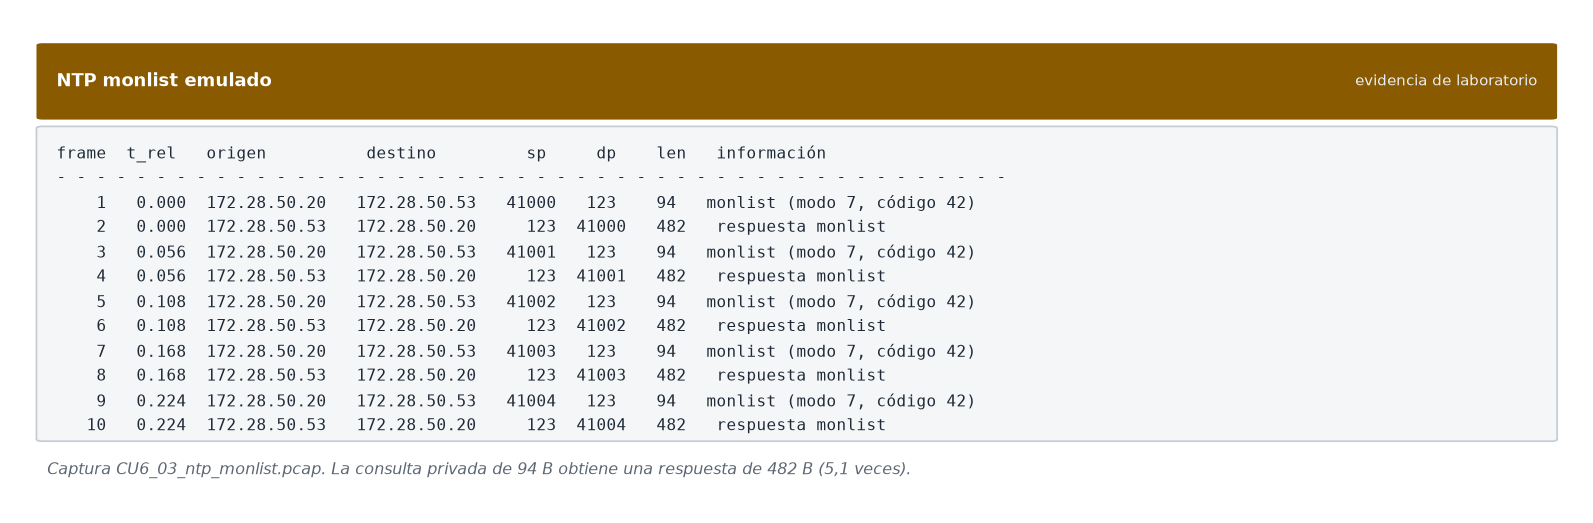
\includegraphics[width=0.98\textwidth]{imagenes/Evidencias CU-6/04_ntp_monlist.png}
	\caption{Consulta y respuesta NTP monlist emuladas (extracto de \texttt{CU6\_03\_ntp\_monlist.pcap}).}
	\label{fig:c6_ntp}
\end{figure}

\begin{figure}[H]
	\centering
	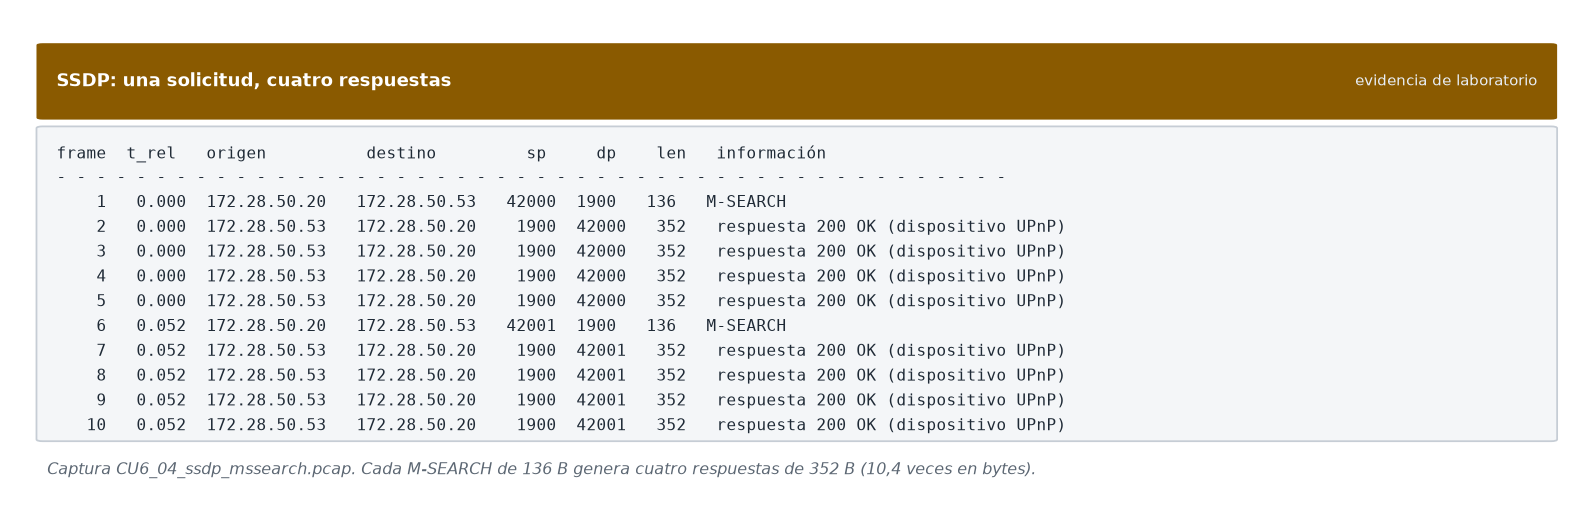
\includegraphics[width=0.98\textwidth]{imagenes/Evidencias CU-6/05_ssdp.png}
	\caption{Una solicitud SSDP y cuatro respuestas (extracto de \texttt{CU6\_04\_ssdp\_mssearch.pcap}).}
	\label{fig:c6_ssdp}
\end{figure}

\begin{figure}[H]
	\centering
	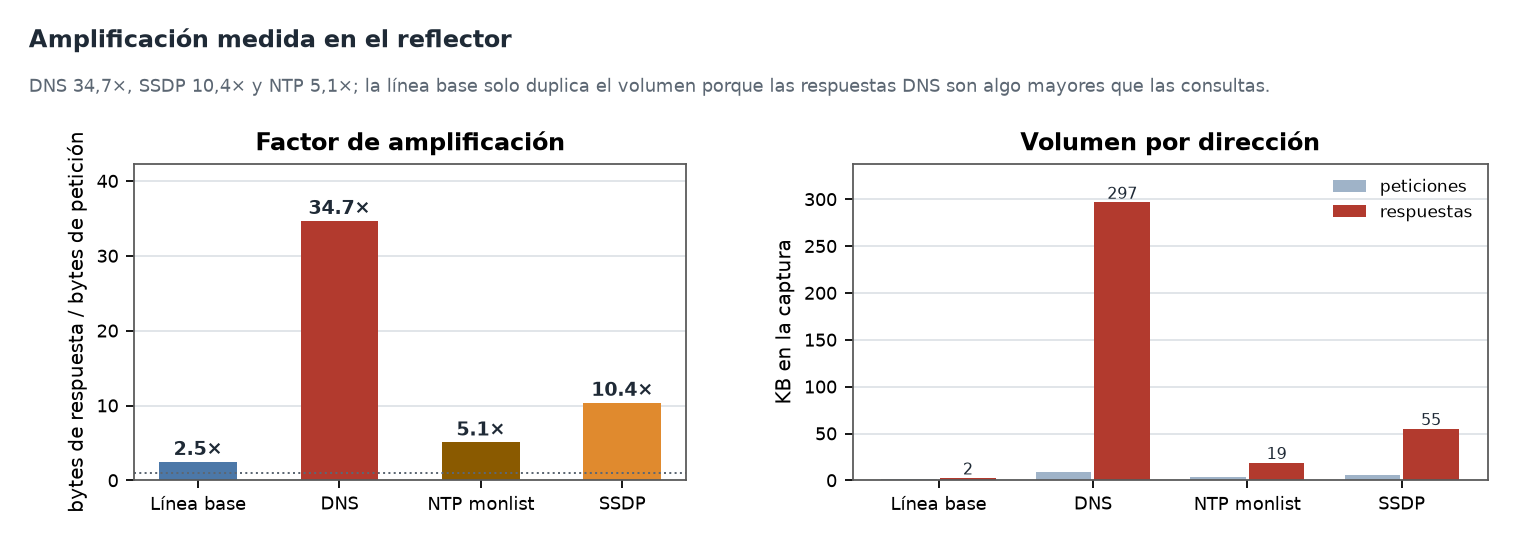
\includegraphics[width=0.96\textwidth]{imagenes/Evidencias CU-6/06_amplificacion.png}
	\caption{Factor de amplificación y volumen por dirección en cada escenario.}
	\label{fig:c6_factor}
\end{figure}

\paragraph{Análisis de resultados.}
La línea base demuestra que la asimetría entre petición y respuesta es normal en DNS: el servidor devuelve más de lo que recibe porque la respuesta incluye el nombre consultado y los registros. Por eso el factor de amplificación solo tiene sentido cuando se compara con el comportamiento esperado del mismo servicio y se acompaña de otra evidencia.

Esa segunda evidencia es la dirección. En la línea base, las respuestas vuelven al mismo host que consultó (\texttt{172.28.50.10}). En las tres fases de amplificación, las respuestas viajan a \texttt{172.28.50.20}, que no envió ninguna consulta. La captura de la víctima lo confirma: 440 tramas y 379.320~bytes recibidos en 11,7~s, con 120 respuestas DNS fragmentadas, 40 respuestas NTP y 160 respuestas SSDP, y cero consultas originadas por el host (Figura~\ref{fig:c6_victima}). La combinación de ambas capturas —reflector y víctima— es la que sostiene la conclusión; ninguna de las dos, por separado, prueba la falsificación del origen.

\begin{figure}[H]
	\centering
	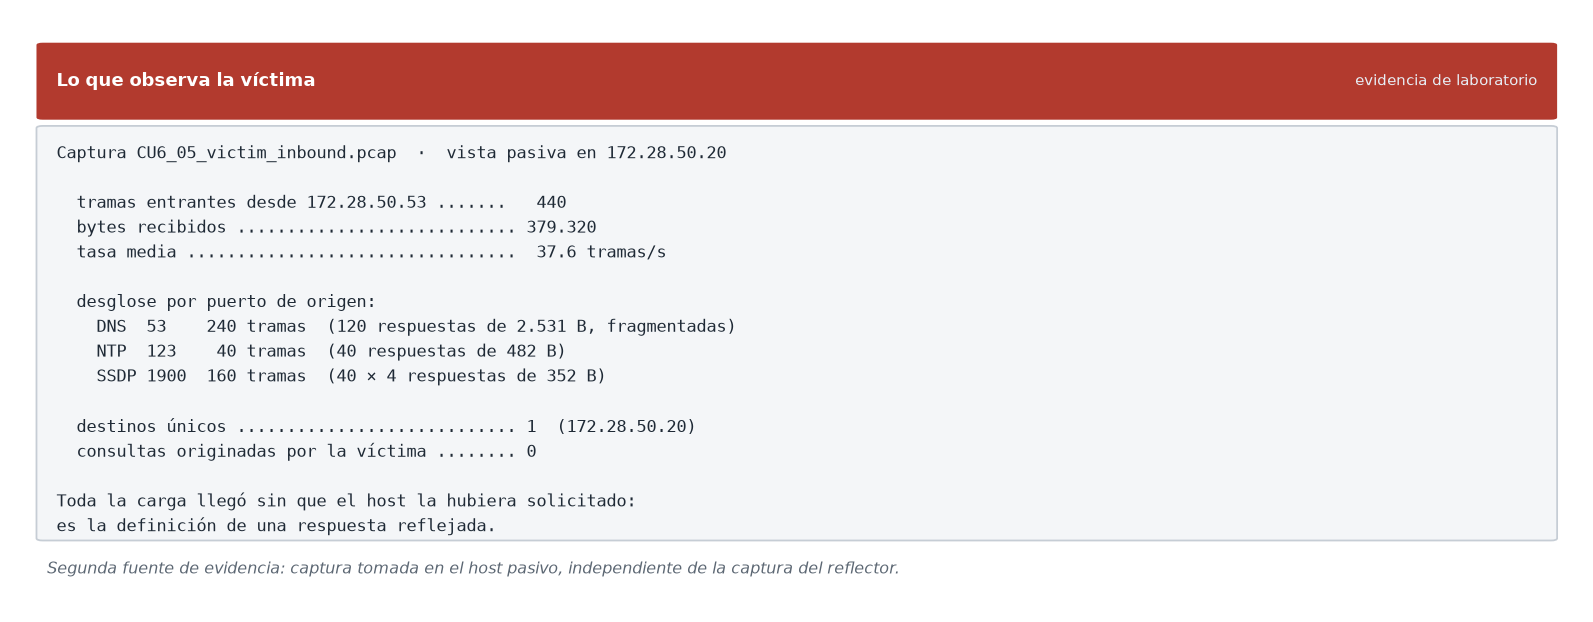
\includegraphics[width=0.98\textwidth]{imagenes/Evidencias CU-6/07_victima.png}
	\caption{Tráfico entrante observado en la víctima, que no originó ninguna consulta.}
	\label{fig:c6_victima}
\end{figure}

La fragmentación es un indicador adicional. Una respuesta DNS de 2.455~bytes no cabe en una trama de 1.500~bytes y se parte en dos; en la captura, las 240 tramas de respuesta corresponden a 120 respuestas fragmentadas. Un IDS que solo inspeccione la primera trama o que descarte fragmentos puede perder el evento, y un analista que cuente tramas en lugar de respuestas puede sobreestimar el número de mensajes. En este caso se reportan ambas cifras de forma explícita.

El tamaño del reflector importa. Los factores medidos dependen de la respuesta configurada: 2.455~bytes de carga DNS, 440~bytes de carga NTP y cuatro respuestas SSDP de 352~bytes en el enlace. En Internet, los factores publicados para DNS superan con frecuencia 30$\times$ y pueden llegar a 50$\times$ o más con respuestas DNSSEC o ANY \parencite{nawrocki2021farside}; los valores del laboratorio son coherentes con esa escala y no pretenden reproducir un ataque real de gran volumen.

\paragraph{Indicadores de detección.}
\begin{itemize}
	\item \textbf{Respuestas no solicitadas:} un host recibe respuestas DNS, NTP o SSDP sin consultas previas registradas.
	\item \textbf{Relación respuesta/petición:} volumen de respuesta muy superior al de petición para un mismo destino y protocolo, comparado con la línea base del servicio.
	\item \textbf{Fragmentación:} respuestas UDP grandes divididas en varios fragmentos IP.
	\item \textbf{NTP modo 7:} peticiones privadas con código 42 (monlist), que ningún cliente legítimo moderno necesita.
	\item \textbf{SSDP repetido:} ráfagas de \texttt{M-SEARCH} desde un mismo origen, cada una con varias respuestas.
	\item \textbf{Concentración de destinos:} muchas respuestas dirigidas a un mismo host y puertos de origen variados.
	\item \textbf{Asimetría de flujo:} el destino recibe mucho más de lo que envía y no tiene conexiones asociadas.
\end{itemize}

\paragraph{Regla de detección propuesta.}
Las reglas se validaron contra las cuatro capturas del reflector. La 1006001 detecta respuestas DNS grandes; la 1006002, la consulta monlist; la 1006003, la ráfaga de \texttt{M-SEARCH}.

\begin{verbatim}
alert udp any 53 -> any any (
  msg:"CU6 respuesta DNS de gran tamano (posible amplificacion)";
  dsize:>1000;
  threshold: type threshold, track by_dst, count 20, seconds 10;
  classtype:attempted-dos; sid:1006001; rev:1;)

alert udp any any -> any 123 (
  msg:"CU6 solicitud NTP monlist (modo 7)";
  content:"|17 00|"; depth:2; content:"|00 2a|"; offset:8; depth:2;
  classtype:attempted-dos; sid:1006002; rev:1;)

alert udp any any -> any 1900 (
  msg:"CU6 rafaga de M-SEARCH SSDP (posible reflexion)";
  content:"M-SEARCH"; depth:8;
  threshold: type threshold, track by_src, count 20, seconds 10;
  classtype:attempted-dos; sid:1006003; rev:1;)
\end{verbatim}

El reprocesamiento produjo cero alertas en la línea base, seis de la regla 1006001 en la fase DNS, cuarenta de la 1006002 en NTP y dos de la 1006003 en SSDP (Figura~\ref{fig:c6_suricata}). La regla 1006001 usa un umbral de veinte respuestas grandes por destino en diez segundos: una respuesta grande aislada no alerta, pero una ráfaga sí. La regla de frecuencia del Caso~2 también se activó en la fase DNS, lo que muestra que una misma señal puede pertenecer a dos casos: ciento veinte consultas en seis segundos son, a la vez, una ráfaga de DNS y el motor de una amplificación.

\begin{figure}[H]
	\centering
	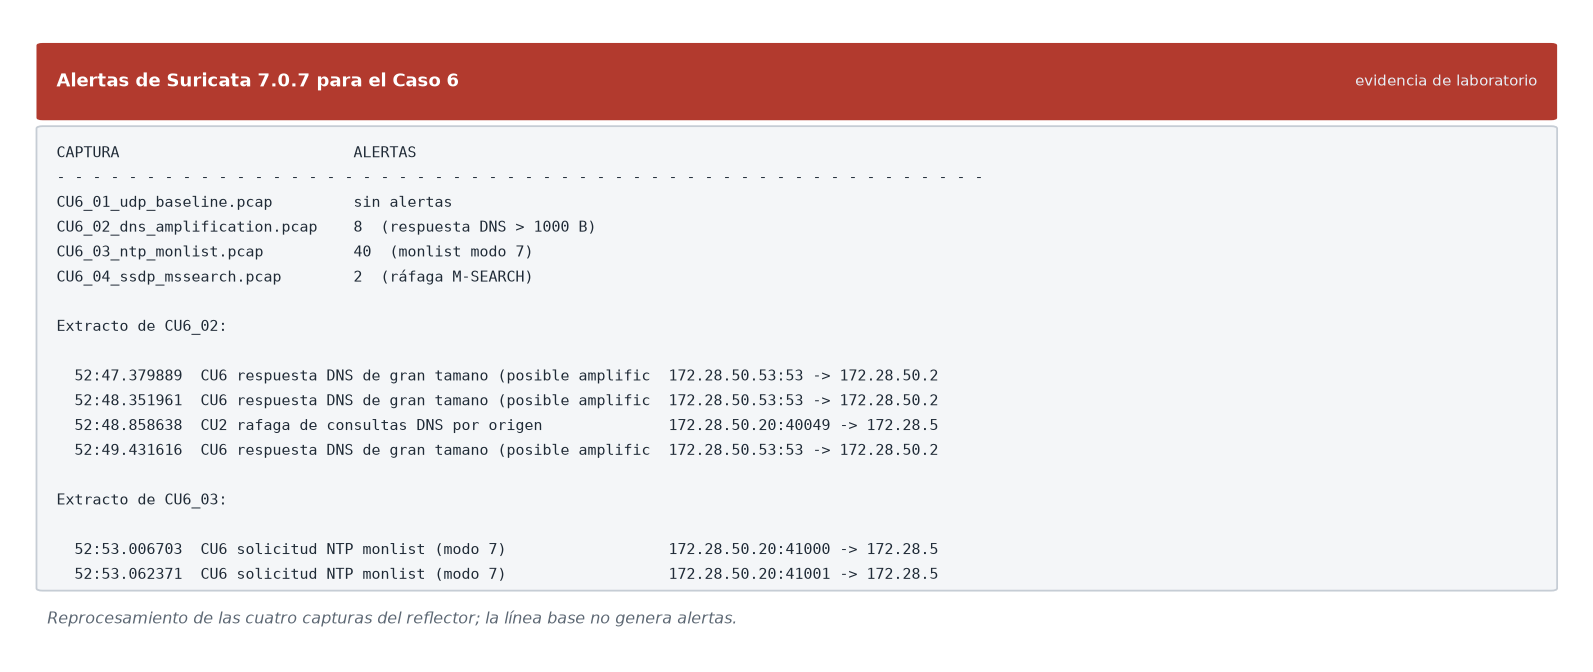
\includegraphics[width=0.98\textwidth]{imagenes/Evidencias CU-6/08_suricata_alertas.png}
	\caption{Alertas de Suricata 7.0.7 al reprocesar las capturas del Caso 6.}
	\label{fig:c6_suricata}
\end{figure}

\paragraph{Mitigación y defensa.}
\begin{itemize}
	\item \textbf{En el servidor:} deshabilitar la recursión abierta y permitirla solo a clientes autorizados; deshabilitar \textit{monlist} y los comandos privados de NTP; restringir SSDP a la red local; aplicar limitación de tasa de respuestas (RRL) y límites de tamaño; apagar los servicios que no se usan.
	\item \textbf{En la red del operador:} filtrado de origen (BCP~38) y unicast reverse path forwarding en el borde; ACL de puertos UDP sensibles; telemetría de flujos para detectar picos por destino; mitigación con \textit{scrubbing} o limitación en el peering.
	\item \textbf{En la red de la víctima:} filtrado de entrada para descartar respuestas no solicitadas y limitación de tasa por destino; sirve para contener el daño, pero no elimina la causa.
	\item \textbf{En la operación:} inventario de servicios UDP expuestos, revisión periódica de configuraciones, pruebas de reflexión solo en laboratorio y coordinación con el proveedor ante un evento sostenido.
	\item \textbf{En la detección:} combinar el tamaño de la respuesta con la ausencia de consulta previa y con la dirección del flujo; una regla de tamaño aislada puede confundir una respuesta DNS legítima grande con un ataque.
\end{itemize}
La causa raíz —la falsificación de origen— solo se corrige en la red que origina el tráfico, que casi nunca es la de la víctima. Por eso los controles se reparten entre el operador del servicio, el proveedor de tránsito y la red de destino.

\paragraph{Preguntas de análisis.}
\begin{enumerate}
	\item \textbf{¿Cómo se diferencia una ráfaga legítima de un patrón de reflexión?}\par
	Por la correlación con la solicitud. En una ráfaga legítima, el host que recibe la respuesta es el mismo que envió la consulta y existe un registro de esa consulta en el cliente o en el resolver; en una reflexión, el destino no envió nada y el origen aparente es una dirección falsificada. Ayudan también el tamaño y la fragmentación de la respuesta, la cantidad de respuestas por petición, la variedad de puertos de origen, la duración y la comparación con la línea base del servicio. En este laboratorio, la prueba decisiva fue la captura de la víctima con cero consultas originadas.
	\item \textbf{¿Qué controles corresponden al servidor y cuáles al proveedor de red?}\par
	Al servidor le corresponden la configuración y el uso: cerrar la recursión, deshabilitar \textit{monlist}, limitar SSDP, aplicar RRL y límites de tamaño. Al proveedor de red le corresponden el filtrado anti-\textit{spoofing} en el origen, la telemetría, la limitación en el peering y la mitigación del volumen. La víctima solo puede filtrar lo que recibe. Ningún control aislado resuelve el problema: sin filtrado de origen, el atacante puede seguir usando cualquier reflector abierto.
\end{enumerate}

\paragraph{Conclusiones.}
\begin{itemize}
	\item Se midió la amplificación de tres protocolos en un entorno aislado: DNS 34,7$\times$, SSDP 10,4$\times$ y NTP 5,1$\times$ en bytes de enlace, con factores sobre la carga de 79$\times$, 13,2$\times$ y 8,5$\times$ respectivamente.
	\item La línea base mostró una asimetría normal de 2,5$\times$: la asimetría por sí sola no es un indicador de ataque.
	\item La captura de la víctima, independiente de la del reflector, confirmó 379.320~bytes entrantes y cero consultas originadas.
	\item La fragmentación de las respuestas DNS fue un indicador visible y, a la vez, una dificultad de conteo que el análisis debió resolver.
	\item Las reglas 1006001, 1006002 y 1006003 detectaron los tres escenarios sin alertar en la línea base; la regla de frecuencia del Caso~2 también se activó, lo que evidencia el cruce entre casos.
	\item Limitaciones: los servicios de NTP y SSDP son emulaciones didácticas, el reflector se configuró deliberadamente abierto, la escala es pequeña y no se reproduce un ataque distribuido ni una red real de terceros.
\end{itemize}

\begin{table}[H]
	\centering
	\caption{Ficha de registro del hallazgo. Caso 6}
	\footnotesize
	\renewcommand{\arraystretch}{1.2}
	\begin{tabularx}{\textwidth}{@{}>{\raggedright\arraybackslash}p{0.23\textwidth} Y@{}}
		\toprule
		\textbf{Campo} & \textbf{Registro} \\ \midrule
		Identificador & Caso 6 (reflexión/amplificación UDP), evidencias \texttt{01\_topologia\_lab.png} a \texttt{08\_suricata\_alertas.png}. Analista: equipo de laboratorio. \\ \hline
		Fecha y hora & 10 de noviembre de 2026, 16:52 (UTC$-$5); \texttt{CU6\_01} a \texttt{CU6\_05}. \\ \hline
		Origen/destino & Origen falsificado \texttt{172.28.50.20}, reflector \texttt{172.28.50.53}, puertos UDP 53, 123 y 1900. \\ \hline
		Observación & 120 consultas DNS, 40 consultas monlist y 40 \texttt{M-SEARCH} con origen falsificado; respuestas de 2.531, 482 y 4~$\times$~352~bytes, respectivamente. \\ \hline
		Hipótesis & La amplificación se reconocerá por una relación respuesta/petición superior a la línea base y por respuestas que llegan a un host que no consultó. \\ \hline
		Validación & Captura del reflector y captura independiente de la víctima: 379.320~bytes entrantes y cero consultas originadas. Suricata: 0, 6, 40 y 2 alertas. \\ \hline
		Severidad & Alta en producción por el volumen y la facilidad de repetición; informativa en el laboratorio aislado. \\ \hline
		Acción & Cerrar la recursión, deshabilitar monlist, restringir SSDP, aplicar RRL y filtrado de origen, y monitorear flujos por destino. \\ \hline
		Integridad & \texttt{CU6\_02}: \texttt{c63ff112\dots0162d63a}; \texttt{CU6\_05}: \texttt{04526293\dots928de546} (SHA-256 truncado; el valor completo está en el Anexo~A). \\
		\bottomrule
	\end{tabularx}
\end{table}
